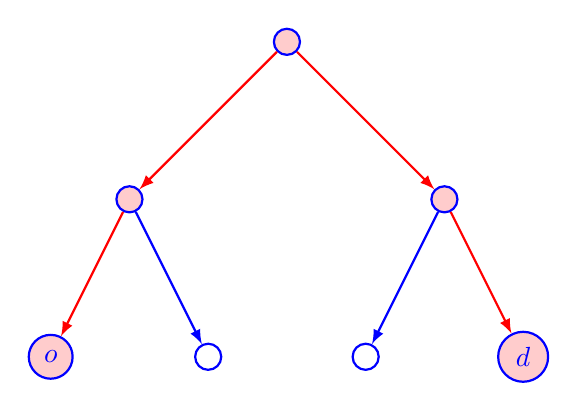
\begin{tikzpicture}[blue, thick]
  \node[draw, circle, fill=red!20] (V1) at (3, 4) {};
  \node[draw, circle, fill=red!20] (V2) at (1, 2) {};
  \node[draw, circle, fill=red!20] (V3) at (5, 2) {};
  \node[draw, circle, fill=red!20] (V4) at (0, 0) {$o$};
  \node[draw, circle] (V5) at (2, 0) {};
  \node[draw, circle] (V6) at (4, 0) {};
  \node[draw, circle, fill=red!20] (V7) at (6, 0) {$d$};

  \draw[-latex, red] (V1) -- (V2);
  \draw[-latex, red] (V1) -- (V3);
  \draw[-latex, red] (V2) -- (V4);
  \draw[-latex] (V2) -- (V5);
  \draw[-latex] (V3) -- (V6);
  \draw[-latex, red] (V3) -- (V7);
\end{tikzpicture}

